\documentclass[tikz,border=0pt]{standalone}
\usepackage{pgfplots}
\usepgfplotslibrary{fillbetween}
\pgfplotsset{compat=1.16}

\definecolor{myBlue}{RGB}{56, 77, 193}

\begin{document}
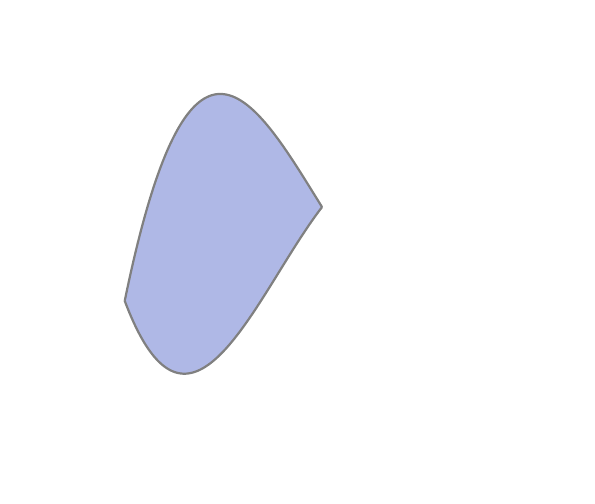
\begin{tikzpicture}
  \def\mystart{-1.1007}
  \def\myend{0.72745}
  \begin{axis}[
    axis lines = none,
    xlabel = \(x\),
    ylabel = \(y\),
    xmin=-2, xmax=3,
    ymin=-3, ymax=3,
    samples=200,
    domain=-3:3,
    no markers,
    ytick={-2,-1,0,1}
    ]
    \addplot[thick, gray, domain=\mystart:\myend] {x^3 - 2*x^2 - x + 2}; % Black line following upper polynomial
    \addplot[thick, gray, domain=\mystart:\myend] {-(x^3) + x^2 + 2*x - 1}; % Black line following lower polynomial
    \addplot[name path=upper, color=blue, opacity=0, thick] {x^3 - 2*x^2 - x + 2}; % Upper polynomial (invisible)
    \addplot[name path=lower, color=red, opacity=0, thick] {-(x^3) + x^2 + 2*x - 1}; % Lower polynomial (invisible)
    \addplot[fill=myBlue, opacity=0.4] fill between[of=upper and lower, soft clip={domain=\mystart:\myend}];
    %\node[color=blue,fill=white] at (axis cs:1.55,2.3) {\(f(x) = x^3 - 2x^2 - x + 2\)}; % Text for the upper function
    %\node[color=red,fill=white] at (axis cs:1.55,-2.3) {\(g(x) = -x^3 + x^2 + 2x - 1\)}; % Text for the lower function
    \%node[white, rotate=90] at (-0.33,0.3) {???};
  \end{axis}
\end{tikzpicture}
\end{document}
